\documentclass{beamer}
\usepackage{etex}
\usepackage[utf8]{inputenc}
\usepackage[T2A]{fontenc}
\usepackage{graphics,graphicx,epsfig}
\usepackage{amssymb,amsfonts,amsthm,amsmath,mathtext,cite,enumerate,float}
\usepackage[english,russian]{babel}
\usepackage[all]{xy}
\usepackage{pgf}
\usepackage[debug,outputdir={docgraphs/}]{dot2texi}
\usepackage{tikz}
\usepackage{scalefnt}
\usepackage{graphicx}
\usepackage{ulem}\normalem
\usetheme{Warsaw}
\usecolortheme{sidebartab}
\usefonttheme[onlylarge]{structurebold}
\setbeamerfont*{frametitle}{size=\normalsize,series=\bfseries}
\setbeamertemplate{navigation symbols}{}
\setbeameroption{show notes}
\setbeamertemplate{itemize items}[circle]
\setbeamertemplate{enumerate items}[circle]
\setbeamertemplate{blocks}[rounded][shadow=false]

\newtheorem{algo}{Алгоритм}
\newtheorem{stat}{Утверждение}
\newtheorem{defin}{Определение}
\newtheorem{theo}{Теорема}

\newcommand{\NBin}[1]{\mathbf{NBin}\ \text{#1}\ }
\newcommand{\NUn}[1]{\mathbf{NUn}\ \text{#1}\ }
\newcommand{\LVar}{\mathbf{LVar}\ }
\newcommand{\LC}{\mathbf{LC}\ }

\begin{document}

\title[Порождение и выбор моделей\hspace{4em}\insertframenumber/\inserttotalframenumber]{Алгоритмы индуктивного порождения и критерии выбора оптимальной существенно нелинейной регрессионной модели}
\author{Г. И. Рудой}
\institute{Московский физико-технический институт \vfill
Факультет управления и прикладной математики \vfill
Кафедра интеллектуальных систем \vfill
Научный руководитель: В. В. Стрижов}
\date{Июнь 2014}

\begin{frame}
  \maketitle
\end{frame}

\begin{frame}{Цель работы}
  \begin{itemize}
  	\item Разработка и анализ алгоритма порождения суперпозиций существенно нелинейных регрессионных моделей.
	  \begin{itemize}
		\item Доказательство существования данной суперпозиции.
		\item Разработка практически реализуемого алгоритма.
	  \end{itemize}
	\item Формулирование и обоснование понятия устойчивости параметров моделей:
	\begin{itemize}
	  \item Критерий выбора моделей.
	  \item Исследование погрешности в измеряемых данных.
	\end{itemize}
  \end{itemize}
\end{frame}

\begin{frame}{Постановка задачи выбора модели}
  Дана выборка
  \[
  D = \{ (\mathbf{x}_i, y_i) \mid i \in \{1, \dots, N\},
			  \mathbf{x}_i \in \mathbb{X} \subset \mathbb{R}^n,
			  y_i \in \mathbb{Y} \subset \mathbb{R} \}.
  \]
  Для множества всех суперпозиций
  \[
  \mathcal{F} = \{ f_r \mid
			  f_r : (\boldsymbol{\omega}, \mathbf{x}) \mapsto y \in \mathbb{Y},
			  r \in \mathbb{N} \},
  \]
  требуется найти индекс $\hat{r}$ такой, что функция $f_{\hat{r}}$ доставляет
  минимум функционалу качества $Q$:
  \[
  \hat{r} = \arg \min_{r \in \mathbb{N}} Q (f_r \mid \boldsymbol{\hat{\omega}_r}, D),
  \]
  \[
  \boldsymbol{\hat{\omega}_r} = \arg \min_{\boldsymbol{\omega} \in \Omega} S(\boldsymbol{\omega} \mid f_r, D).
  \]
\end{frame}

\begin{frame}{Символьная регрессия}
  Аппроксимация выборки некоторой формулой:
  \[
  y = \sin x_1^2 + 2x_2.
  \]

  Методы:
  \begin{itemize}
	\item Генетические алгоритмы [Koza1998].
	\item Аналитическое программирование [Zelinka2008, Webb2010].
  \end{itemize}
\end{frame}

\begin{frame}{Проблемы аналитического программирования}
  \frametitle{Проблемы аналитического программирования}

  \begin{itemize}
	\item Порождение рекурсивных суперпозиций:
	  \[
	  f = y + f (x, y).
	  \]
	\item Несоответствие арности функций числу и типам аргументов:
	  \[
	  f = \sin (x, y, z).
	  \]
	\item Несовпадение областей определения и значений:
	  \[
	  f = \sqrt{-x^2}.
	  \]
	\item Порождение слишком сложных суперпозиций.
  \end{itemize}
\end{frame}

\begin{frame}{Постановка теоретической задачи}
  \frametitle{Постановка теоретической задачи}

  Пусть $G = \{ g_1, \dots, g_l \}$~--- множество данных порождающих
  функций; для каждой $g_i \in G$ заданы:
  \begin{itemize}
	\item функция (например, $\sin$, $\cos$, $\times$),
	\item арность функции и~порядок следования аргументов,
	\item тип аргументов ($\text{dom} g_i$) и тип значения ($\text{cod} g_i$) функции,
	\item область определения $\mathcal{D} g_i \subset \text{dom} g_i$ и~область
	  значений $\mathcal{E} g_i \subset \text{cod} g_i$.
  \end{itemize}
  Требуется:
  \begin{itemize}
	\item построить алгоритм, за конечное число итераций
	  порождающий любую конечную суперпозицию данных примитивных функций,
	\item oценить сложность полученного алгоритма,
	\item доказать полноту полученного алгоритма.
  \end{itemize}
\end{frame}

%\begin{frame}{Постановка теоретической задачи}
%  \frametitle{Постановка теоретической задачи}
%
%  Для функции $f(x_1, x_2) = \log_{x_1} x_2$:
%  \[
%	\text{dom} f = \mathbb{R} \times \mathbb{R},
%  \]
%  \[
%	\text{cod} f = \mathbb{R},
%  \]
%  \[
%	\mathcal{D} f = \{ (x_1, x_2) \mid x_1 \in (0; 1) \cup (1; +\infty), x_2 \in (0; +\infty) \},
%  \]
%  \[
%	\mathcal{E} f = (-\infty; +\infty).
%  \]
%\end{frame}

%\begin{frame}{Дерево суперпозиции}
%  \frametitle{Дерево суперпозиции}
%  Каждой суперпозиции $f$ сопоставлено дерево $\Gamma_f$.
%
%  \begin{itemize}
%	\item В~вершинах $V_i$ дерева $\Gamma_f$ находятся соответствующие
%	  порождающие функции $g_s, s = s(i)$.
%	\item Число дочерних вершин у некоторой вершины $V_i$ равно арности
%	  соответствующей функции $g_s$.
%	\item Порядок смежных некоторой вершине $V_i$ вершин соотвествует порядку
%	  аргументов соответствующей функции $g_{s(i)}$.
%	\item В~листьях дерева $\Gamma_f$ находятся свободные переменные $x_i$
%	  либо числовые параметры $\omega_i$.
%	\end{itemize}
%\end{frame}

\begin{frame}[fragile]
  \frametitle{Дерево суперпозиции}

  \begin{figure}[h]
	\centering
	\begin{tikzpicture}
	  \scalefont{2}
	  \tikzstyle{n} = [draw, inner sep=2pt, fill=red!20]
		\begin{dot2tex}[dot,options=-tmath,scale=0.3]
		  digraph G1 {
			node [shape="circle",style="n"];
			
			Plus [label="\bullet + \bullet"];
			Sin [label="\sin \bullet"];
			Ln [label="\ln \bullet"];
			X1 [label="x_1"];
			Frac [label="\div"];
			Pow [label="\bullet^{\bullet}"];
			X2 [label="x_2"];
			N3 [label="3"];
			N2 [label="2"];

			Plus -> Sin;
			Sin -> Ln;
			Ln -> X1;

			Plus -> Frac;
			Frac -> Pow;
			Frac -> N2;

			Pow -> X2;
			Pow -> N3;
		  }
		\end{dot2tex}
	  \end{tikzpicture}
  \end{figure}

  \[
  f = \sin (\ln x_1) + \frac{x_2^3}{2}.
  \]
\end{frame}

\begin{frame}{Индуктивное порождение суперпозиций}
  \frametitle{Алгоритм индуктивного порождения суперпозиций}
	
	\[
	G = G_b \cup G_u; X = \{ x_1, \dots, x_n \}.
	\]

	\begin{enumerate}
	  \item Инициализация:
		\[
		  \mathcal{F}_0 = X,
		\]
		\[
		  \mathcal{I} = \{ (x, 0) \mid x \in X \}.
		\]
	  \item Вспомогательные множества:
		\[
		  U_i = \{ g_u \circ f \mid g_u \in G_u, f \in \mathcal{F}_i \},
		\]
		\[
		  B_i = \{ g_b \circ (f, h) \mid g_b \in G_b, f, h \in \mathcal{F}_i \}.
		\]
	  \item $\mathcal{F}_{i+1} = \mathcal{F}_i \cup U_i \cup B_i$.
	  \item $\mathcal{I} = \mathcal{I} \cup (f, i + 1)$, если $f$ не присутствует
		в $\mathcal{I}$.
	\end{enumerate}

	Множество всех возможных суперпозиций $\mathcal{F} = \cup_{i=0}^{\infty} \mathcal{F}_i$.
\end{frame}

%\begin{frame}
%  \frametitle{Функции многих переменных и параметрические модели}
%
%  \begin{itemize}
%	\item Для множества функций $G_n$ арности $n$ вспомогательное множество $H_i^n$:
%	  \[
%	  H_i^n = \{ g \circ (f_1, f_2, \dots, f_n) \mid g \in G_n, f_j \in \mathcal{F}_i \},
%	  \]
%	  тогда $\mathcal{F}_{i+1} = \mathcal{F}_i \cup_{n=0}^{n_{max}} H_i^n$ (кроме того, $U_i \equiv H_i^1$, а $B_i \equiv H_i^2$).
%
%	  Множество всех возможных суперпозиций $\mathcal{F} = \cup_{i=0}^{\infty} \mathcal{F}_i$.
%	\item Изменим вспомогательные множества:
%	  \[
%	  U_i = { g_u \circ (\alpha f + \beta) },
%	  \]
%	  \[
%	  B_i = { g_b \circ (\alpha f + \beta, \psi h + \phi) }.
%	  \]
%	  Переменные $\alpha, \beta, \psi, \phi$~--- параметры модели.
%  \end{itemize}
%\end{frame}

\begin{frame}
  \frametitle{Оценка сложности и стохастический алгоритм}
  
  \begin{theo}
	Предложенный алгоритм породит любую конечную суперпозицию за конечное число шагов.
  \end{theo}

  \begin{theo}
	Пусть в множестве примитивных функций $G$ содержится $l_p$ функций арности
	$p > 1$ и ни одной функции арности $p + k \mid k > 0$, и имеется $n > 1$
	независимых переменных. Тогда справедлива следующая оценка количества
	суперпозиций, порожденных предложенным алгоритмом после $k$-ой итерации:
	\[
	| \mathcal{F}_k | = \mathcal{O} (l_p^{\sum_{i=0}^{k-1} p^i} n^{p^k}).
	\]
  \end{theo}

  \begin{itemize}
	\item Суперпозиции порождаются случайным образом.
	\item Наименее удачные суперпозиции изменяются с сохранением структуры.
	\item Наиболее удачные суперпозиции комбинируются.
  \end{itemize}
\end{frame}

\begin{frame}
  \frametitle{Критерий выбора моделей}

  \[
  Q_f = \frac{1}{1 + S_f} \left(\alpha + \frac{1 - \alpha}{1 + \text{exp} (\frac{C_f}{\beta} - \tau)}\right).
  \]
  \begin{itemize}
	\item $S_f$~--- функционал ошибки.
	\item $C_f$~--- сложность модели.
	\item $\alpha$~--- коэффициент влияния штрафа за сложность, $0 \ll \alpha < 1$,
	\item $\beta$~--- коэффициент строгости штрафа за сложность, $\beta > 0$,
	\item $\tau$~--- коэффициент, характеризующий желаемую сложность модели.
  \end{itemize}
\end{frame}

\begin{frame}{Постановка задачи исследования устойчивости}
  Дано:
  \begin{itemize}
   \item Обучающая выборка $D$:
     \[
	   D = \{ \mathbf{x}_i, y_i \} \mid i \in \{ 1, \dots, \ell \}.
     \]
   \item Семейство $\mathcal{F}$ параметрических функций $f = f(\mathbf{x}, \boldsymbol{\omega})$.
   \item Функционал качества $S$:
     \[
       S = S (f (\cdot, \boldsymbol{\omega}), D) \mid f \in \mathcal{F}, \quad S \rightarrow \mathop{\min}\limits_{\boldsymbol{\omega}}
     \]
  \end{itemize}
  
  Требуется:
  \begin{itemize}
    \item Исследовать зависимость $\hat{\boldsymbol{\omega}} = \mathop{\arg \min}\limits_{\boldsymbol{\omega}} S$ от вариации $D$.
    \item Выбрать оптимальную модель согласно зависимости от вариации $D$.
    \item Проверить возможность экспертного применения $f$ при данной вариации $D$.
  \end{itemize}
\end{frame}

\begin{frame}{Известные результаты}
  \begin{itemize}
    \item Случай линейной регрессии:
      \[
        y_i = ax_i + b + \xi_i \mid i \in \{ 1, \dots, n \}, \xi_i \in \mathcal{N} (0, \sigma).
      \]
    \item Влияние пертурбаций на решения оптимизационных задач [Bonnans1998].
    \item Верхние границы ошибок в SVM [Vapnik2000].
    \item Сравнение стабильности и обобщающей способности при варьировании обучающей выборки [Bousquet2002].
    \item Вычислительная стабильность интерполяции [Higham2003].
    \item Стабильность алгоритмов кластеризации [Luxburg2009].
    \item Малые изменения входных данных в сетях глубокого обучения [Szegedy2014].
  \end{itemize}
\end{frame}

\begin{frame}{Предлагаемый алгоритм}
  \begin{enumerate}
    \item Фиксируется параметрическая модель $f \in \mathcal{F}$:
      \[
        f = f(\mathbf{x}, \boldsymbol{\omega}) \in \mathcal{F}.
      \]
    \item Начальный оптимальный вектор параметров:
      \[
        \hat{\boldsymbol{\omega}}_f(D) = \mathop{\arg \min}\limits_{\boldsymbol{\omega}_f} S(f, D).
      \]
  \end{enumerate}
\end{frame}

\begin{frame}{Предлагаемый алгоритм}
  \begin{enumerate}
    \setcounter{enumi}{2}
    \item Варьируется выборка:
      \begin{align*}
        \acute{D}(\Sigma^{\mathbf{x}}, \boldsymbol{\sigma}^y) = \{ \mathbf{x}_i + \boldsymbol{\xi}^{\mathbf{x}}_i, y_i + \xi^y_i \mid\ &i \in 1, \dots, \ell;\\
        & \boldsymbol{\xi}^{\mathbf{x}}_i \sim \mathcal{N}(0; \boldsymbol{\sigma}^{\mathbf{x}}_{i \cdot}); \\
        & \xi^y_i \sim \mathcal{N}(0; \sigma^y_i) \},
      \end{align*}
      где $\Sigma^{\mathbf{x}} = \Vert \boldsymbol{\sigma}^{\mathbf{x}}_{ij} \Vert$.
    \item Оптимальный вектор параметров для варьированной выборки $\acute{D}$:
      \[
    		\hat{\boldsymbol{\omega}}_f (\acute{D} (\Sigma^{\mathbf{x}}, \boldsymbol{\sigma}_y)) = \mathop{\arg \min}\limits_{\boldsymbol{\omega}_f} S (f (\cdot, \boldsymbol{\omega}_f), \acute{D} (\Sigma^{\mathbf{x}}, \boldsymbol{\sigma}_y)).
      \]
    \item Разность с начальным оптимальным вектором $\hat{\boldsymbol{\omega}}_f$:
      \[
        \Delta\hat{\boldsymbol{\omega}}_f(\acute{D} (\Sigma^{\mathbf{x}}, \boldsymbol{\sigma}_y) ) = \hat{\boldsymbol{\omega}}_f(D) - \hat{\boldsymbol{\omega}}_f (\acute{D} (\Sigma^{\mathbf{x}}, \boldsymbol{\sigma}_y))
      \]
     \item Шаги 3-5 повторяются $N$ раз:
      \[
        \acute{\mathcal{D}}_N (\Sigma^{\mathbf{x}}, \boldsymbol{\sigma}_y) = \{ \acute{D}_1 (\Sigma^{\mathbf{x}}, \boldsymbol{\sigma}_y), \dots, \acute{D}_N (\Sigma^{\mathbf{x}}, \boldsymbol{\sigma}_y) \}.
      \]
   \end{enumerate}
\end{frame}

\begin{frame}{Предлагаемый алгоритм}
  \begin{enumerate}
    \setcounter{enumi}{5}
    \item Вычисляется стандартное отклонение каждой компоненты вектора параметров:
      \[
        \sigma_{\omega_i} = \text{stddev} ((\Delta\hat{\boldsymbol{\omega}}_f)_i).
      \]
    \item Устойчивость $i$-го параметра относительно компоненты $j$ описания:
      \[
        T^N_f(i, j, \Sigma^{\mathbf{x}}, \boldsymbol{\sigma}_y) = \frac{\frac{\sigma_{\omega_i}}{\hat{\omega}_i}}{r(\{\frac{\boldsymbol{\sigma}^\mathbf{x}_{k j}}{\mathbf{x}_{k j}}\}_{k = 1}^{\ell})}.
      \]
  \end{enumerate}
  
  $r$ выбирается экспертом, например:
  \begin{itemize}
    \item $r(a_1, \dots) = a_1$~--- для равных относительных погрешностей;
    \item $r(a_1, \dots, a_{\ell}) = \frac{\sum_{i = 1}^{\ell} a_i}{\ell}$~--- средняя относительная погрешность.
  \end{itemize}
  
  $T > 1 \Rightarrow$ относительная погрешность параметра больше относительной
  погрешности в данных.
\end{frame}

\begin{frame}{Случай независимых коэффициентов}
  \begin{theo}[Рудой]
    Пусть стандартные отклонения $j$-ых компонент $\mathbf{x}$ одинаковы:
    \[
      \forall i_1, i_2, j: \sigma_{i_1 j}^{\mathbf{x}} = \sigma_{i_2 j}^{\mathbf{x}}.
    \]
    Пусть коэффициенты $\omega_i$ попарно не коррелируют:
    \[
      \forall i_1, i_2: \text{Cov} (\omega_{i_1}, \omega_{i_2}) = 0.
    \]
    Тогда для достаточно малых $\sigma_{ij}^\mathbf{x}$:
    \begin{align*}
      \{ \sigma_{\omega_i} (\boldsymbol{\sigma}_{\cdot 1}, \boldsymbol{\sigma}_{\cdot 2}, \dots, \boldsymbol{\sigma}_{\cdot |\mathbf{x}|}) \}^2 &=
        \{ \sigma_{\omega_i} (\boldsymbol{\sigma}_{\cdot 1}, 0, 0, \dots, 0) \}^2 + \nonumber \\
        & + \{ \sigma_{\omega_i} (0, \boldsymbol{\sigma}_{\cdot 2}, 0, \dots, 0) \}^2 + \nonumber \\
        & + \dots + \nonumber \\
        & + \{ \sigma_{\omega_i} (0, 0, \dots, 0, \boldsymbol{\sigma}_{\cdot |\mathbf{x}|} \}^2 + O(\sigma_{ij}^{\boldsymbol{x}}).
      \label{eq:pypha_variance}
    \end{align*}
  \end{theo}
\end{frame}

\begin{frame}{Вычислительный эксперимент: дисперсия полимеров}
  Дано:
  \begin{itemize}
    \item $D_j = (\lambda_i^j, n_i^j) \mid i \in \{ 1, \dots, 17 \}, j \in \{ 1, 2 \}.$
    \item Экспертные предположения.
  \end{itemize}
  
  Требуется:
  \begin{itemize}
    \item $n_j = n_j(\lambda).$
    \item Оценить адекватность $n_1 (\lambda) - n_2 (\lambda)$.
  \end{itemize}
\end{frame}

\begin{frame}{Порождение моделей}
  \[
    Q(f) = \frac{1}{1 + S(f)} \left(\alpha + \frac{1 - \alpha}{1 + \text{exp} (\frac{C(f)}{\beta} - \tau)}\right).
  \]

  \begin{figure}[h]
    \vspace{-20pt}
    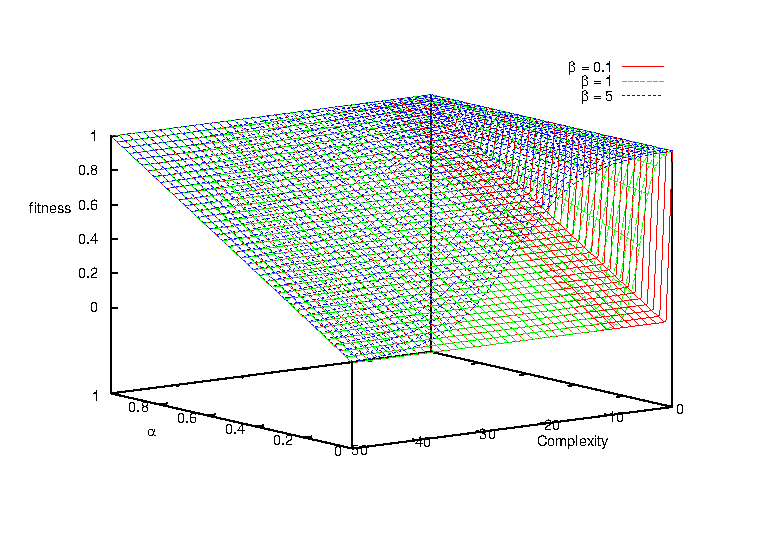
\includegraphics[scale=0.8]{figs/fitness.eps}
    \vspace{-30pt}
  \end{figure}
\end{frame}

\begin{frame}{Порожденные модели}
  Две модели:
  \begin{itemize}
    \item $n_1(\lambda) = 1.34 + \frac{3.54 \cdot 10^3}{\lambda^2} + \frac{2 \cdot 10^3}{\lambda^4}$.
    \item $n_2(\lambda) = 1.34 + \frac{11.6}{\lambda} + \frac{17.37}{\lambda^2} + \frac{0.0866}{\lambda^3} + \frac{2.95 \cdot 10^{-4}}{\lambda^4} + \frac{8.54 \cdot 10^{-7}}{\lambda^5}.$
  \end{itemize}
  
  \begin{table}[h]
    \centering
    \begin{tabular}{| c | c | c | l | c | c | c |} \hline
  	$\tau$	& Суперпозиция		& $MSE$					& $C(f)$		& $Q(f)$ \\ \hline
	10	  	& $n_1$		  		& $2.4 \cdot 10^{-8}$	& 13			& 0.095	\\ \hline
	30		& $n_2$				& $3.9 \cdot 10^{-9}$	& 31			& 0.031	\\ \hline
    \end{tabular}
  \end{table}
  
  Экспертное мнение: $n_2$ некорректна, нечетных степеней быть не может.
\end{frame}

\begin{frame}{Устойчивость моделей}
\begin{table}[h]
    \centering
    \begin{tabular}{c | c}
	  $n_1$ & $n_2$ \\ \hline
	  \includegraphics[scale=0.4]{{figs/even/p1.txt_coeff0.dat}.eps} & \includegraphics[scale=0.4]{{figs/all/p1.txt_coeff0.dat}.eps} \\
    \end{tabular}
    \caption{Графики стандартного отклонения первого коэффициента для моделей $n_1$ и $n_2$.}
  \end{table}
  
  Устойчивость второй модели в $\approx 40$ раз хуже.
\end{frame}

\begin{frame}{Устойчивость моделей}
  \begin{table}[h]
    \centering
    \begin{tabular}{l | c c c}
	  $n$ & $\omega_1$ & $\omega_2$ & $\omega_3$ \\ \hline
	  1 & \includegraphics[scale=0.25]{{figs/even/p1.txt_coeff0.dat}.eps} & 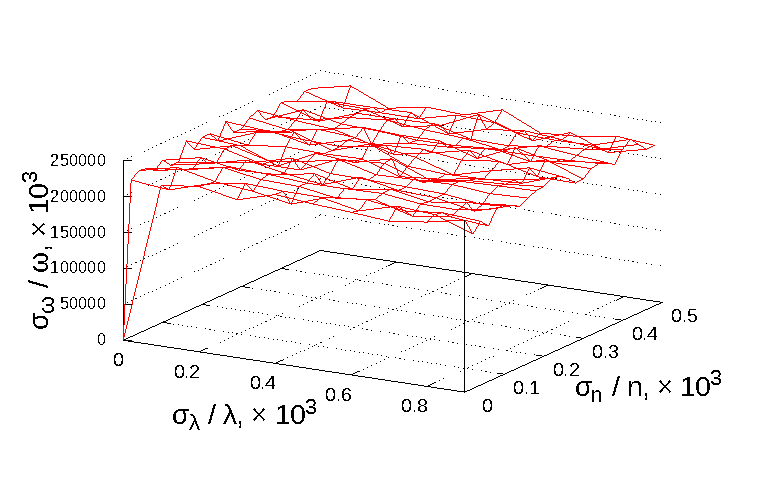
\includegraphics[scale=0.25]{{figs/even/p1.txt_coeff1.dat}.eps} & 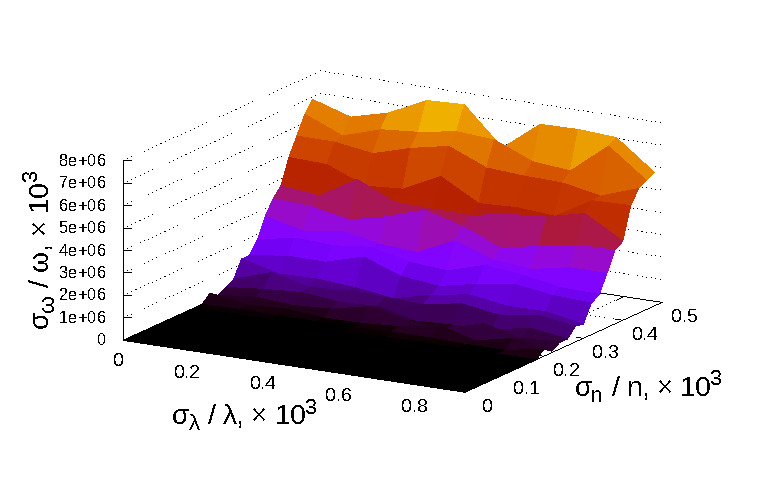
\includegraphics[scale=0.25]{{figs/even/p1.txt_coeff2.dat}.eps} \\
	  2 & 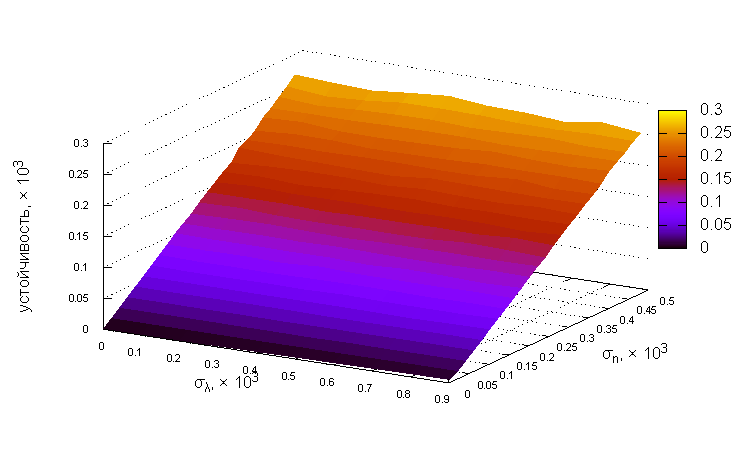
\includegraphics[scale=0.25]{{figs/all/p2.txt_coeff0.dat}.eps} & 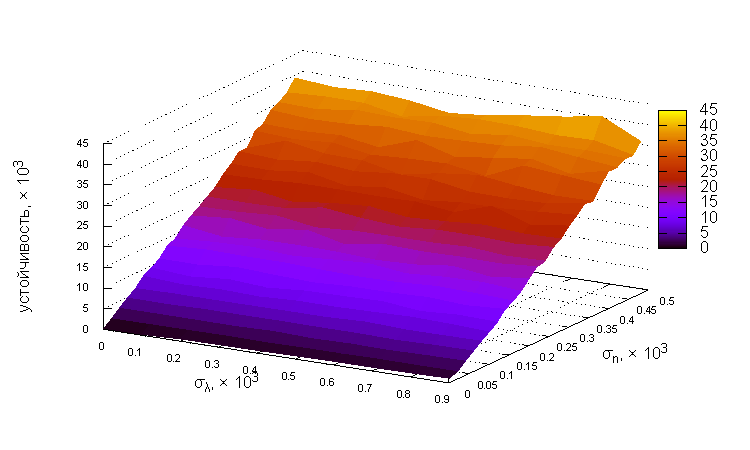
\includegraphics[scale=0.25]{{figs/all/p2.txt_coeff1.dat}.eps} & 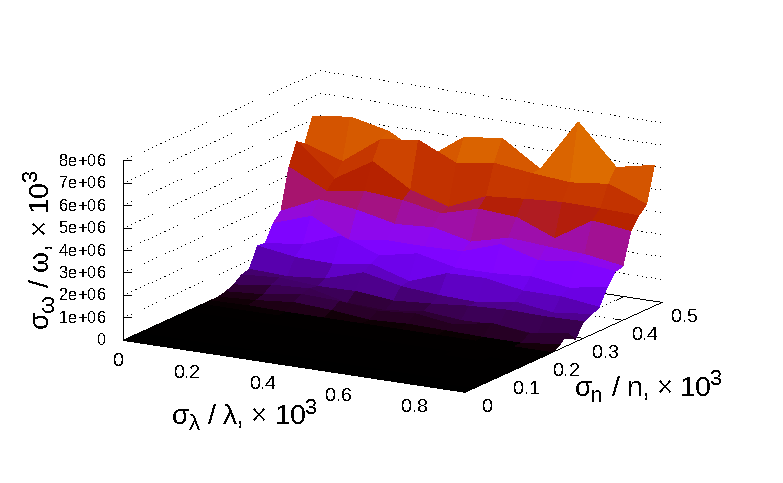
\includegraphics[scale=0.25]{{figs/all/p2.txt_coeff2.dat}.eps}
    \end{tabular}
    \caption{Графики стандартного отклонения первых трех коэффициентов для моделей $n_1$ и $n_2$.}
  \end{table}
\end{frame}

\begin{frame}{Разделяемость моделей}
  \begin{table}[h]
    \centering
    \footnotesize
    \begin{tabular}{| l | c | c | c | c |} \hline
  	Полимер		& $\omega_1$		& $\omega_2$		& $\omega_3$		& MSE	\\ \hline
      1			& 1.34946		& 3558.95		& 1924.33		& $2.2 \cdot 10^{-8}$		\\ \hline
      2			& 1.34047		& 3118.84		& 1578.59		& $1.4 \cdot 10^{-8}$		\\ \hline
  	Разность	& $6.71 \cdot 10^{-3}$	& $1.41 \cdot 10^{-1}$	& $2.2 \cdot 10^{-1}$	&	\\ \hline
    \end{tabular}
    \caption{Значения коэффициентов для модели $n_1$ и их относительная разность.}
  \end{table}
  
  \begin{table}[h]
    \centering
    \footnotesize
    \begin{tabular}{| l | c | c | c |} \hline
	  Коэфф.	& $(2 \cdot 10^{-4}; 2 \cdot 10^{-5})$	& $ (6 \cdot 10^{-4}; 6 \cdot 10^{-5}) $	& $ (9 \cdot 10^{-4}; 2 \cdot 10^{-4}) $ \\ \hline
	  1		& $1.22 \cdot 10^{-5}$					& $ 3.59 \cdot 10^{-5} $					& $ 1.19 \cdot 10^{-4} $		\\ \hline
	  2		& $1.48 \cdot 10^{-3}$					& $ 4.38 \cdot 10^{-3} $					& $ 1.44 \cdot 10^{-2} $		\\ \hline
    \end{tabular}
    \caption{Значения стандартного отклонения для коэффициентов модели $n_1$ для первого полимера в зависимости от относительных дисперсий $(\frac{\sigma_{\lambda}}{\lambda}, \frac{\sigma_n}{n})$.}
  \end{table}
  
  Модели разделимы: $\omega_1^1 - \omega_1^2 = 6.71 \cdot 10^{-3} >> \sigma_{\omega_1} = 1.19 \cdot 10^{-4}$.
\end{frame}

\begin{frame}{Лагранжева интерполяция}
  Существенно переобученная модель:
  \[
    L(x) = \prod_{i = 0}^\ell y_i \prod_{j = 0, j \neq i}^\ell \frac{x - x_j}{x_i - x_j},
  \]
  \begin{table}[h]
    \centering
    \begin{tabular}{c c}
      \includegraphics[scale=0.45]{{figs/lagrange/p1.txt_coeff0.dat}.eps}	& 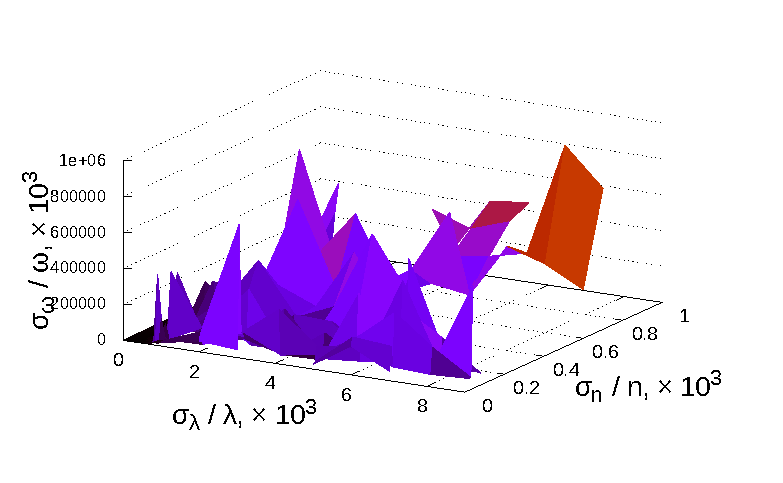
\includegraphics[scale=0.45]{{figs/lagrange/p1.txt_coeff0.dat_small}.eps}
    \end{tabular}
    \caption{Поверхность стандартного отклонения коэффициента $\omega_0$.}
  \end{table}
\end{frame}

\begin{frame}{Публикации и работы}
  \scriptsize
  \begin{itemize}
    \item Г. И. Рудой, В. В. Стрижов. Алгоритмы индуктивного порождения суперпозиций для аппроксимации измеряемых данных --- <<Информатика и её применения>> --- 2013. --- № 7. --- С. 44--53.
    \item Г. И. Рудой, В. В. Стрижов. Индуктивное порождение суперпозиций в задачах нелинейной регрессии --- <<Машинное обучение и анализ данных>> --- 2011. --- № 2. --- С. 140-155.
    \item Г. И. Рудой. Анализ устойчивости существенно нелинейных регрессионных моделей к погрешностям в измеряемых данных.~--- <<ЖВММФ>> (направлено в журнал).
    \item Г. И. Рудой. О возможности применения методов Монте-Карло в анализе нелинейных регрессионных моделей.~--- <<СибЖВМ>> (направлено в журнал).
    \item Г. И. Рудой. Исследование устойчивости существенно нелинейных регрессионных моделей к погрешностям в обучающей выборке.~--- Труды 56-й научной конференции МФТИ. Раздел <<Управление и прикладная математика>>, т. 1, с. 102-103. Москва, Долгопрудный, 2013.
    \item Г. И. Рудой. Устойчивость существенно нелинейных регрессионных моделей и метод её исследования.~--- Труды международной конференции студентов, аспирантов и молодых ученых <<ЛОМОНОСОВ-2014>>, секция <<Математическая статистика и ее приложения>>. Москва, 2014.
  \end{itemize}
\end{frame}

\begin{frame}{Результаты}
  \begin{itemize}
    \item Предложен алгоритм, порождающий все возможные суперпозиции заданной сложности за конечное число шагов, и получена оценка его сложности.
    \item Описан стохастический алгоритм порождения существенно нелинейных суперпозиций и приведены результаты вычислительного эксперимента на синтетических данных.
    \item Предложено понятие устойчивости параметров модели.
    \item Обосновано использование понятия устойчивости параметров модели в качестве критерия выбора моделей.
    \item Продемонстрировано использование понятия устойчивости для анализа применимости экспертных моделей.
    \item Исследованы различные регрессионные модели и связь предложенного критерия с критериями ошибки и сложности модели.
  \end{itemize}
\end{frame}

\end{document}